% ---------------------------------------------------------------------
% ---------------------------------------------------------------------
% ---------------------------------------------------------------------
\part{Introduction and literature review}
\chapter[Introduction, contents and aims of the thesis]{Introduction, contents and aims of the thesis}



% ---------------------------------------------------------------------
% ---------------------------------------------------------------------
\section{Introduction}
\label{sec:Intro}
Data sets have experienced a rapid growth in size and complexity during the last years, and biology and biomedicine have been no exception \parencite{marx2013biology, costa2014big}. Few decades ago, a typical data set consisted in dozens of variables, and a large data set was one with some few hundreds of variables. Nowadays, the different 'omic' technologies have evolved producing data sets ranging from hundreds of variables, in the case of specific panels or targeted analyses, to thousands or even hundreds of thousands of variables for untargeted or whole genome analyses. A specific characteristic of 'omic' data sets, compared to data sets from other disciplines is their heterogeneous nature. Individual variability is huge and experiments have to be repeated many times to reach conclusions \parencite{lay2006problems}. This has lead to the so called "reproducibility crisis", which considers that many research findings could be false \parencite{ioannidis2005most, begley2015reproducibility}. In fact, as shown in \autoref{figura32}, some studies have estimated that more than 70\% of published works in the field of biology may be not reproducible \parencite{baker20161}.

Among the causes for lack of reproducibility, the most prominent ones are the use of inadequate statistical methods, the misuse of adequate statistical methods and the misunderstanding of statistical results \parencite{ioannidis2017statistical, gagnier2017misconceptions, diong2018poor}. There is also an inertia to continue using the same outdated methods that have been used during the last 30 years \parencite{leek2017five}. These issues are prevalent in all scientific branches, but in biology, and most specifically in the field of 'omic' data, they are critical because of the enormous variability in the data (both technical and biological), the large number of variables and the prevailing low sample sizes. It is still very common to find publications in top journals where no corrections for multiple comparisons have been applied after performing hundreds of tests or using statistical methods such as the \textit{t test} without even considering their assumptions (normality and homocedasticity) \parencite{marino2014use, eklund2016cluster}. During the last decades, a wide array of statistical methods have been specifically developed to deal with the issues and hurdles present when analyzing 'omic' data sets, but their adoption has been pretty slow in most fields. In the following chapters, the different methods for analyzing 'omic' data will be presented and critically reviewed before presenting a new method for the analysis of multi-way arrays that also implements variable selection.

\begin{figure}[hbtp]
	\centering
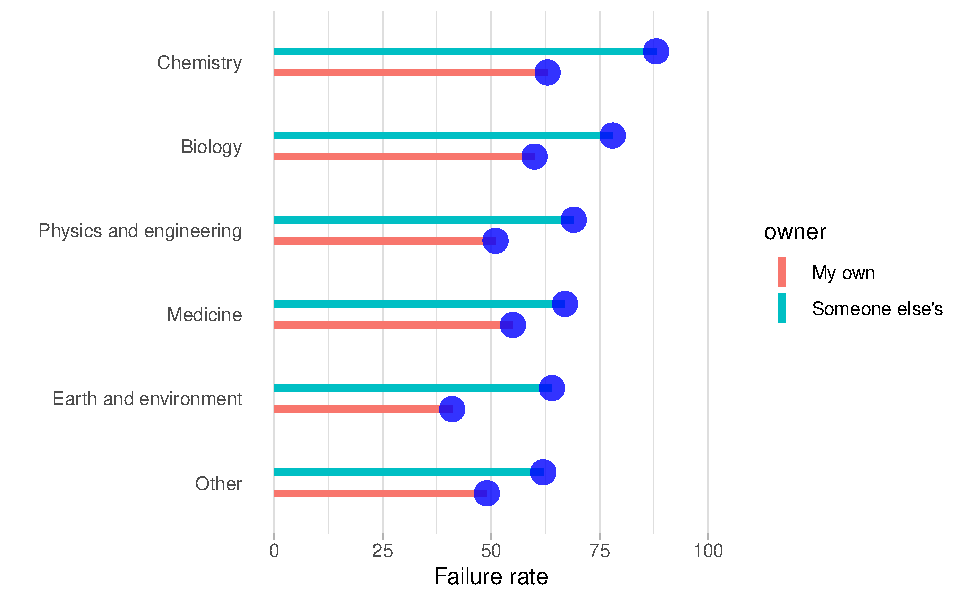
\includegraphics[width=0.9\textwidth]{figura32.pdf}
\caption{Reproducibility problems in different branches of science (data from \cite{baker20161})}
\label{figura32}
\end{figure}

\section{Characteristics of 'omic' data}
\label{sec:charomicdata}
The word "omics" makes reference to the study of some characteristics of different families of biological molecules, such as genes, proteins, etc. \parencite{palsson2002silico}. The basic aspect of the 'omic' approaches is that a complex system can be understood more thoroughly if considered as a whole. Thanks to this approach, the advances that have been achieved in the last decades in the understanding of the different biological processes are huge, and today the future of medicine and biology cannot be understood outside the view of the different 'omics' approaches \parencite{van2018role}. In few years, 'omics' technologies have given us an unimaginable deep knowledge of many cellular processes and pathways, helping the scientific community to make huge progresses in the understanding of living systems. Each year new technologies are developed allowing for the gathering of more information, increasing the resolution of the analyses and improving the precision of the determinations. As emerging fields, the different 'omics' are still expanding and defining themselves but, in a general view, 'omic' data can be classified according to the nature of the elements being analyzed. Following this approach, 5 different fields can be delimited (\autoref{figura01}), \parencite{horgan2011omic, 2018iv}:

\vspace{10pt}

\begin{itemize}
    \item Genomics: Focused at the structure, function, evolution and mapping of genomes, that is, the complete set of DNA of an organism.
    \item Epigenomics: Studies the complete set of epigenetic reversible modifications of the genome, which regulate expression.
    \item Transcriptomics: Focused at the whole set of RNA transcripts of an organism, that is, the expression of an organism's genes.
    \item Proteomics: Focused at the whole set of proteins produced or modified by an organism. Proteomics studies protein composition, structure and activity.
    \item Metabolomics: Studies metabolites in a biological entity, which are the end products of cellular processes.
\end{itemize}

\begin{figure}[htbp]\centering
		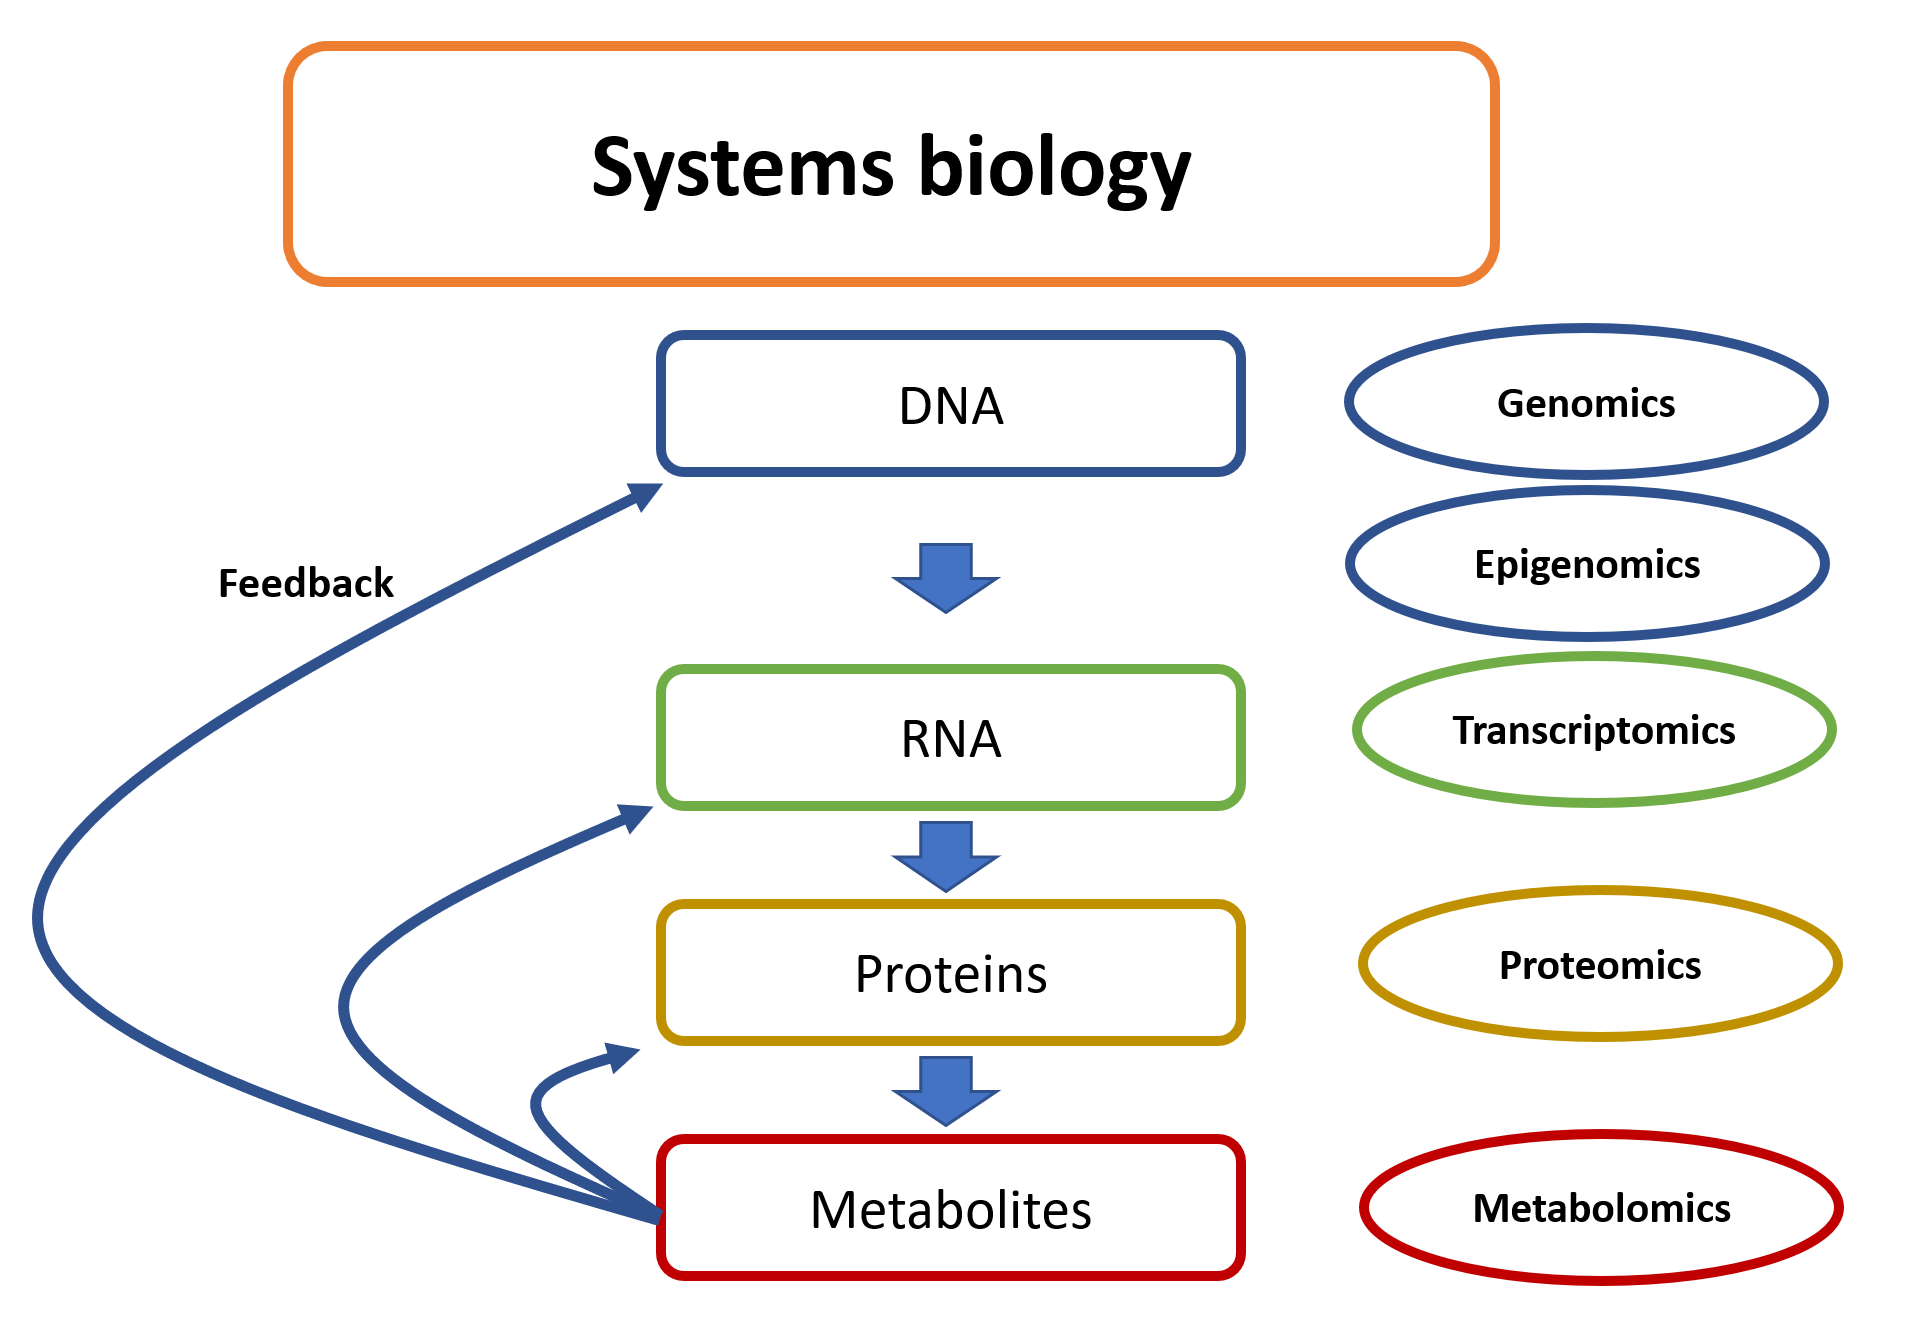
\includegraphics[width=.7\textwidth]{figura01}
		\caption{Different 'omic' technologies and their relationship}
		\label{figura01}
	\end{figure}



\subsection{Metabolomic data}
The term '\textit{metabolome}' is used to address the entire set of metabolites present in an organism and '\textit{metabolomics}' is defined as the comprehensive and quantitative analysis of all metabolites of the biological system under study \parencite{fiehn2001combining}. Metabolomics studies the downstream products of the so called "omics cascade" presented in \autoref{figura01}, so its information is influenced by the actions of genomic, epigenomic, transcriptomic and proteomic mechanisms. Because of this, metabolomics is the closest approximation to phenotype among all 'omic' technologies, thus providing  more information about the actual status of the organism than the other 'omic' technologies \parencite{beger2016metabolomics}. 

In general metabolomic studies can be classified as targeted or untargeted depending on whether the researcher measures and quantifies a specific set of known metabolites or the largest possible number of metabolites contained in a biological system \parencite{orevsivc2009metabolomics}. 
Among all 'omic' technologies, metabolomics is the most complex and heterogeneous in terms of chemical diversity. More specifically, targeted metabolomic studies focus on accurate identification and quantification of a defined set of metabolites in biological samples which was predetermined by the scientific question formulated by the researcher or, in some cases, by the size of metabolite library that is available in the software used for the analyses. On the other hand, untargeted metabolomics focuses on measuring and comparing as many signals as possible in a biological samples, and then assigning these signals to specific metabolites by using annotation databases such as HMDB \parencite{wishart2007hmdb} and Metlin \parencite{smith2005metlin}. It is important to mention that a significant portion of the detected signals cannot be identified as the metabolome is not fully annotated \parencite{viant2017close}. A typical raw data spectrum of a metabolomics analysis is presented in \autoref{figura37}.

\begin{figure}[htbp]\centering
		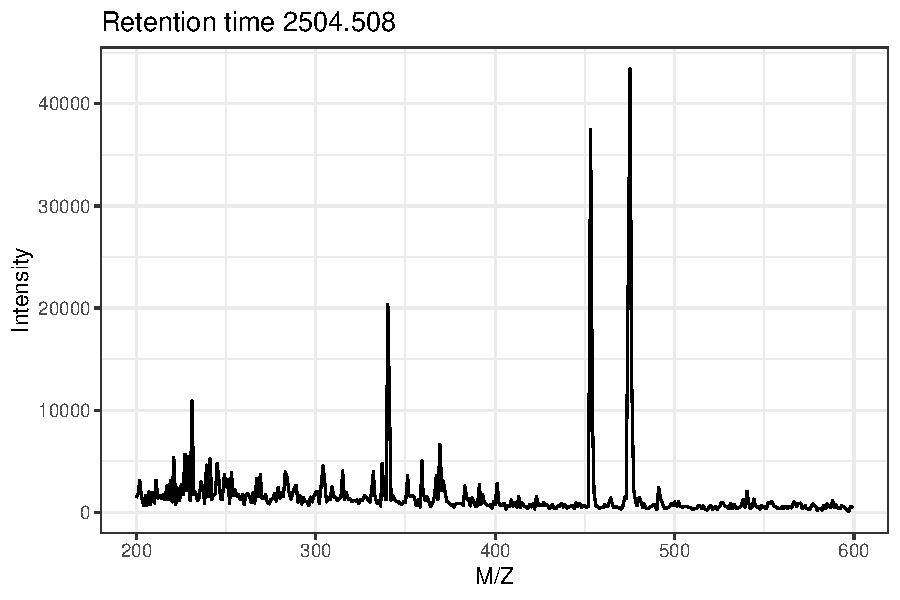
\includegraphics[width=.7\textwidth]{figura37.pdf}
		\caption{Raw spectrum of a metabolomics analysis}
		\label{figura37}
	\end{figure}

In genomics, epigenomics and transcriptomics, measurement procedures are reasonably standardized. This is not the case in metabolomics, with many different technologies being used, which lead to different study designs and different produced data types \parencite{moco2007metabolomics}. The commonly used analytical techniques for metabolomic studies are nuclear magnetic resonance (NMR), spectroscopy and mass spectrometry \parencite{buscher2009cross}. Another specific hurdle of metabolomics is the identification of the metabolites in untargeted analyses. Many of the metabolites found in an untargeted analysis can not be identified, because the data bases for associating a specific mass and retention time to a concrete metabolite are still very immature \parencite{mathew2013metabolomics}. In fact, identification of unknowns is considered as the bottleneck of untargeted metabolomics \parencite{bingol2018recent}.
In any case, although heterogeneous, metabolomic data share a common set of properties which define their most important characteristics for their statistical analysis:

\begin{itemize}
    \item High correlation among variables
    \item Complex pre-processing of the signal to obtain the data
    \item High range of detection values among variables (i.e., some metabolites are found in very small concentrations and others are found in very high concentrations)
    \item Variables (metabolites) found in one analysis are not guaranteed to be found in a subsequent analysis (i.e., lack of reproducibility).
\end{itemize}

All these properties add to the difficulty of analyzing metabolomic data, and will be further developed in the following sections.

